\documentclass[conference]{IEEEtran}
\IEEEoverridecommandlockouts
% The preceding line is only needed to identify funding in the first footnote. If that is unneeded, please comment it out.
\usepackage{cite}
\usepackage{amsmath,amssymb,amsfonts}
\usepackage{algorithmic}
\usepackage{url}
\makeatletter
\g@addto@macro{\UrlBreaks}{\UrlOrds}
\makeatother
\usepackage{graphicx}
\usepackage{siunitx}
\usepackage{commath}
\usepackage{textcomp}
\usepackage{xcolor}
\def\BibTeX{{\rm B\kern-.05em{\sc i\kern-.025em b}\kern-.08em
    T\kern-.1667em\lower.7ex\hbox{E}\kern-.125emX}}
\begin{document}

\title{MECH0010 Case Study Report}

\author{\IEEEauthorblockN{Candidate number: NCWT3}}

\maketitle

\begin{abstract}
This document is a piece of coursework for the Control and Instrumentation module - UCL Mechanical Engineering Department. It seeks to describe the characteristics of a real-world control system, which uses transducers and feedback control. I have chosen a CPU cooler as my control system, commonly found in laptops and PCs.
\end{abstract}

\begin{IEEEkeywords}
control, instrumentation, feedback system, closed loop control
\end{IEEEkeywords}

\section{Product overview}
The product chosen is a CPU cooler called the Intel Thermal Solution, designed for Intel processors. The part number of the CPU cooler is E97379-003 and there are three manufacturers: Delta, Foxconn and Nidec \cite{b1}. 

The purpose of the Intel Thermal Solution is to provide cooling to the processor. During operation, the processor outputs heat energy, which must be drawn away from the chip to prevent overheating and damage to the processor and surrounding components. This is achieved through the use of a heat-sink and fan assembly. The heat sink is attached to the processor via mounting hardware on the motherboard. A film of thermal paste is also added in between the heat sink and the processor to aid thermal conduction. On top of the heat sink is an impeller, which passes air through the fins of the heat sink, drawing heat energy away. This keeps the CPU cool and prevents overheating. Cooling the processor allows for more performance to be extracted from the processor before overheating occurs. The CPU fan is connected to the motherboard, from which it receives power and a control signal. 

Feedback control is used here to control the speed of the fan. The fan does not need to run at the maximum possible speed at all times because the processor's thermal output is not constant, varying with processor load. As the fan also makes audible noise and consumes power whilst in use, it is desirable to be able to have the fan run at lower speeds when possible. The feedback loop in this system looks at the temperature of the processor and sets the fan speed accordingly. When the processor is in high-performance mode, the fan speed can be increased and when the processor is idling, it can be reduced. 
\section{Feedback system}
The goal of the feedback system is to provide the system with the information on the current temperature of the system. It is important to measure the actual temperature of the CPU as simply calculating the expected temperature based on processor load is not sufficient. Factors such as air temperature, airflow, humidity, dust and other environmental factors can all cause the temperature of the CPU to fluctuate. With this information, the closed loop system can make adjustments to the fan speed based. For example, on particularly hot days, the cooler may need to run at higher speeds to achieve the same amount of heat exchange. 
\begin{figure}[tbhp]
    \centering
    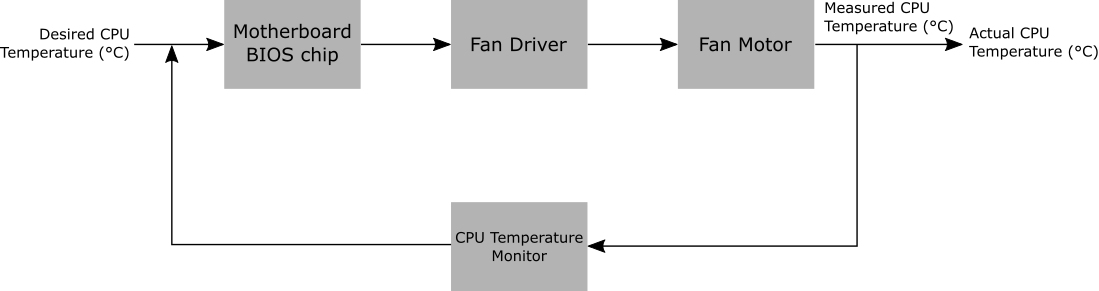
\includegraphics[width=0.489\textwidth]{../img/figure1.png}
    \caption{System block diagram}
\end{figure}
\section{Transducers in feedback system}
The transducer used in our system is part of the processor to which the Thermal Solution is attached. Intel processors measure the temperature of each core by measuring the forward voltage drop of a silicon diode on the chip. This is usually a bipolar junction transistor and the forward voltage drop is temperature dependent. This dependence is described as follows by Widlar \cite{b2} \cite{b7}:
\begin{multline}
    V_{BE} = V_{G0} \left(1-\frac{T}{T_0}\right) + V_{beo}\left(\frac{T}{T_0}\right) + \\\left(\frac{nKT}{q}\right)\ln\left(\frac{T_0}{T}\right) + \left(\frac{KT}{q}\right)\ln\left(\frac{IC}{IC_0}\right) \label{widlar}
\end{multline}
where:
\begin{itemize}
    \item $n$ is a device-dependent constant
    \item $q$ is the charge on an electron
    \item $K$ is Boltzmann's constant
    \item $V_{beo}$ is the bandgap voltage at temperature $T_0$ and current $IC_0$
    \item $V_{G0}$ is the bandgap voltage at absolute zero
    \item $T$ is the temperature in \si{\kelvin}
\end{itemize}
The voltage is measured at two different currents and inputted into \eqref{widlar}, giving us a simplified equation:
\begin{equation}
    \Delta V_{BE} = \left(\frac{KT}{q}\right)\ln\left(\frac{IC_1}{IC_2}\right)
    \label{bandgap}
\end{equation}
Looking at a similar silicon temperature sensor to the one used in a CPU chip (NXP PCT2075), we can look at the data sheet to find how accurate the sensor typically is. The power supply range is from \SI{2.7}{\volt} to \SI{5.5}{\volt}. This gives us temperatures ranging from between \SI{-55}{\celsius} to \SI{+125}{\celsius}. Within this temperature range, the accuracy of the temperature reading is $\pm$\SI{1}{\celsius} between \SI{-25}{\celsius} to \SI{+100}{\celsius} and $\pm$\SI{2}{\celsius} between \SI{-55}{\celsius} to \SI{+125}{\celsius} \cite{b3}. 

The analogue output is converted with an 11-bit ADC that offers a temperature resolution of \SI{0.125}{\celsius}. The measurement is made every \SI{100}{\milli\second} and takes \SI{28}{\milli\second} to convert into bit data. The data is stored in the temperature register and can be read at any time. The register contains two 8-bit data bytes: one Most Significant Byte and one Least Significant Byte. The first significant bit is used as a positive (0) - negative (1) indicator and the other 10 significant bits are used to store the temperature data; the rest of the bits are not relevant to the temperature reading. For example, 011 1111 0001 converted from binary to decimal is 1009. This then needs to be multiplied with \SI{0.125}{\celsius} to get our temperature value, in this case being \SI{126.125}{\celsius}.

A difference between the NXP chip and the transducer on a CPU chip are the activation states of the chips. The NXP chip has a temperature at which it activates ($T_{ots}$ and stays activated and then a reset temperature ($T_{hys}$ hysteresis factor). Compared to a CPU chip, there is only an upper temperature limit, above which the CPU will decrease its clock speed and even reduce its $VCC$ to avoid thermal damage. On an Intel i7-4790k chip, this temperature is \SI{100}{\celsius} (TCC activation temperature) \cite{b4}. The temperature is always monitored, when power is being received to the processor.

This temperature data is read by the motherboard BIOS chip, which is in charge of controlling the fan. The Intel Thermal Solution utilises a four-pin fan design: 
\begin{itemize}
    \item Pin 1 - Black wire: Ground
    \item Pin 2 - Yellow wire: Supply voltage
    \item Pin 3 - Green wire: Tachometer signal
    \item Pin 4 - Blue wire: Pulse-width-modulation signal
\end{itemize}
Pulse-width-modulation allows us to vary the RPM of the fan. By switching the fan's motor on and off rapidly, we can use the fan's mass inertia to rotate the fan at a certain RPM. Here, the PWM signal controls how long the motor is activated for any particular cycle. An ideal tachometer signal is compared to the tachometer signal from pin 3 (which measures the actual rotation of the fan). The PWM can then be adjusted accordingly to bring the RPM to the desired level - dictated by the current temperature of the CPU. This is a feedback loop of its own but will not be explored further in this report. 
\section{Alternative transducers}
An alternative transducer that can be used (and is used for testing purposes on Intel chips) is a thermocouple. This is attached to the integrated heat spreader by machining a groove to the geometric centre of the heat spreader. This thermocouple gives a different set of temperature readings (called $T_{case}$) than the silicon temperature sensors as they are in different positions. As the silicon sensors are embedded in the actual die of the CPU, they are closer to the source of heat than the thermocouple, which is only attached to the heat spreader. This results in the $T_{case}$ temperatures being lower than the core temperatures (which are called junction temperatures $T_{j}$).

A thermocouple operates on the principle of joining two different metals at both ends (junctions). One junction is for measurement and the other is for reference. As the temperature rises or falls at the measuring junction, a voltage is generated. This is directly related to the temperature and can be converted by the reference with an appropriate table of values \cite{b5}. However, since this method of measurement requires altering the chip, it is unsuitable for use in the design environment of the product.

Other transducers which could be used include a thermistor, which operates on the principle of resistance changing with temperature. They are durable, small and affordable. However, the nature of their output is non-linear and they are best suited to measuring a single point of temperature within a limited temperature range \cite{b6}. Their non-linear output would require there to be additional signal processing to extract the temperature data. 

A silicon bandgap temperature sensor is the most suitable transducer in this system. As explored previously we do not need to add any additional components to the chip, resulting in an extremely compact package - important for a processor. They also provide a suitable degree of accuracy over a wide range of temperatures and have a linear output, allowing for easier signal processing. 
\section{Expected nature of signal output from transducer}
The signal output from our silicon temperature sensor is expected to be a linear signal, as defined by \eqref{bandgap}, as long as we keep the ratios of the currents the same. However, as with any system, a totally linear output is not received. Going back to Widlar's formula in \eqref{widlar}, we can think of the terms to be arranged as such \cite{b7} \cite{b8}:
\begin{multline}
    V_{BE} = \textrm{(sum of linear temp terms) } + \\\textrm{ (sum of non-linear temp terms)}
\end{multline}
Widlar showed that the non-linear terms were relatively small and will be considered later. We need to define a base voltage, which is a linear function of temperature, $V_b = C_1 \times T$, where $C_1$ is a constant. The emitter voltage is $V_e = V_b - V_{be}$. Substituting into \eqref{widlar}:
\begin{equation}
    V_e = C_1 T - V_{G0} \left(1 - \frac{T}{T_0}\right) - V_{beo}\left(\frac{T}{T_0}\right) \label{widlar2}
\end{equation}
If we then define $V_e$ being equal to $C_2$ at $T=T_0$, we can solve for $C_1$:
\begin{equation}
    C_1 = \frac{V_{beo} + C_2}{T_0}
\end{equation} 
Substituting this value for $C_1$ in \eqref{widlar2}:
\begin{equation}
    V_e = C_2 \frac{T}{T_0} + V_{G0} \frac{T-T_0}{T_0}
\end{equation}
Differentiating with respect to $T$: 
\begin{equation}
    \frac{\dif V_e}{\dif T} = \frac{C_2 + V_{G0}}{T_0}
\end{equation}
This equation tells us that if we adjust $V_b$ to give $V_e = C_2$ at our chosen $T_0$, the rate of change of $V_e$ with respect to temperature is a constant, independent of $V_b$ or $V_{be}$. Let us choose to take $V_e = C_2 = 0$ at $T_0 = \SI{0}{\celsius}$. The bandgap of silicon at \SI{0}{\kelvin} is typically \SI{1.22}{\volt} \cite{b8}. Our equation reduces to:
\begin{equation}
    \frac{\dif V_e}{\dif T} = \frac{V_{G0}}{273.15} = \SI{4.47}{\milli\volt\per\celsius}
\end{equation}
If we want to be able to trim our system at ambient temperatures, we need only to trim $V_e$ to be equal to \SI{4.47}{\milli\volt\per\celsius} for each degree of displacement from \SI{0}{\celsius}.

As stated previously, the non-linear terms although small are not totally negligible and are found to be quadratic for positive temperatures. Tsividis \cite{b8} \cite{b9} showed that another non-linear term is the bandgap voltage, $V_0$, with respect to temperature. It also causes non-linear terms to become significant under temperatures of \SI{0}{\celsius}. The sum of these non-linear error terms follows an approximate square-law. These can be compensated by a circuit which introduces a square-law current. 

Taking this raw voltage data from our transistor, we can use the aforementioned 11-bit ADC to convert our temperature data into a bit data, storable on memory. 
\section{Costs}
The CPU fan is bundled with Intel chips such as the i3, i5 and i7, and is thus factored into the price of those processors. However, Intel's amazon page does offer the Intel Thermal Solution E97379-001 for purchase as a standalone unit for \$8.99 (excluding shipping) \cite{b13}. 

A data sheet showing the 2D sketches of the Intel Thermal Solution is provided by Intel and breaks down the individual components on the Intel Thermal Solution. It comprises of a simple metal heat sink, a wiring loom, a small amount of thermal paste, an integrated plastic fan/motor assembly, and the plastic mounts. The fan/motor assembly is expected to be the most expensive component of the system. The impeller is made from plastic and is manufactured with a simple moulding process. The motors are designed for use in the Intel Thermal Solution only and are not sold as a separate part. Motors sold online as a standalone part are not a useful comparison, as the motors produced for the CPU fan are manufactured with much different economies of scale. 

The cost of the transducer itself is negligible. As there are billions of transistors on a CPU chip, incorporating one for temperature control comes at little to no extra cost for the manufacturer. Some extra cost will be introduced due to the fact that some circuity to compensate for the non-linearity of the sensor and the calibration circuits must be included. We can also factor the cost of the ADC into our system. The cost of the previously mentioned NXP chip ranges from £0.57 per unit to £0.17 per unit depending on the amount purchased \cite{b10}. Compared to thermistor ICs (£0.5-£2) and thermocouples (£2-£10), these silicon chips provide good value for money \cite{b11} \cite{b12}. 
\section{Accuracy of feedback system}
The feedback system provides a relatively degree of accuracy. Considering the temperature sensitivity of the CPU, they are designed to be able to run at high temperatures for long periods of time (\SI{80}{\celsius} - \SI{100}{\celsius}). The CPU also only reaches such high temperatures under considerably heavy load (100\% sustained loads). Numerous fail-safes are built into the processor to prevent heat damage to the chip. The first of these fail-safes is dynamic frequency control, which reduces the performance of the chip by reducing the clock speed - reducing the thermal output. This temperature is usually in the range of \SI{90}{\celsius} - \SI{105}{\celsius}. On an Intel i7-4790k processor, the Thermal Control Circuit Activation Temperature is defined as \SI{100}{\celsius} \cite{b5}. The second fail-safe is clock modulation, which reduces the thermal output by around 50\% by modulating the clocks on a 30-50\% clock cycle \cite{b5}. A final fail-safe in the form of a complete processor shutdown occurs at \SI{130}{\celsius}, which is designed to be well above the normal operational range of the CPU \cite{b5}. Hence, we can see that our silicon temperature sensor can provide an adequate degree of accuracy for the system. An inaccuracy of $\pm$\SI{1}{\celsius} will not affect the operation of the CPU in normal use cases, as the temperature is not hot enough to affect performance (through the activation of on-board fail-safes). Under heavy loads, the CPU may utilise its fail-safes to prevent overheating, however temperatures of \SI{100}{\celsius} can be maintained by the CPU and the stated inaccuracies will not damage the chip.  
\section{Limitations and improvements}
Some of the limitations of the feedback system include the amount of energy the Intel Thermal Solution can transfer away from the chip, and the calibration and compensation circuits of the silicon temperature sensors. Cooling of the chip allows us to "overclock" the CPU. This involves increasing the clock speeds of the CPU, increasing performance. In order to do this we must make sure that there is enough thermal overheard. Therefore, we must have a more powerful cooling solution. To increase the amount of energy that is transferred away from the chip, we can design a larger heatsink/one can that transfer heat more efficiently, utilise a more thermally conductive material, increase the size of our impeller (and subsequently the size of the motor powering the fan) to increase airflow. However, all these solutions can only cool the processor to a theoretical maximum of ambient temperature. Employing solutions such as water-cooling or oil submersion can help us reach this theoretical maximum. These solutions can transfer heat energy away from the CPU much more effectively, however as they still use radiators to exchange heat energy with air, they are inevitably limited. Aftermarket air-cooling solutions can be anywhere from two times to ten times more expensive \cite{b14}, and liquid cooling solutions can be ten times to 25 times more expensive than the Intel Thermal Solution \cite{b15}. Solutions such as liquid nitrogen cooling also exist, ridding us of the ambient temperature limit, but are extremely impractical for this use case. 

To improve the accuracy of our silicon temperature sensors, we could utilise more complex circuits to account for the non-linear changes in voltages when there is a temperature change. However, the added complexity of the circuits do not provide much additional benefit. One such example is to utilise SiCr thin-film resistors, as they have better temperature coefficient matching. Another example is to design an array of transistors which compensate for the leakage currents of each transistor. These can be become significant at high temperatures (\SI{+250}{\celsius}). As this is outside the operational range of our system, we can opt to not include such a circuit (which would require doubling the number of transistors used for the temperature measurement) \cite{b8}. Our 11-bit ADC also provides a high degree of precision for our temperature measurements. CPUs can rapidly change in temperature with frequent spikes in activity; the sampling rate of \SI{10}{\hertz} allows our system is able to rapidly respond to these changes in temperature. 

The designers have decided not to include the following improvements in the design as to keep the cost of the Intel Thermal Solution low. Designed as a base level cooling solution, more effective cooling solutions exist for those wishing to push their processors to the limit of their performance. For the average consumer, the Intel Thermal Solution is an effective cooler. The temperature sensors inside the chip have adequate systems in place to prevent overheating with reliable transducers to measure the state of the system. Further engineering to improve the accuracy of the transducers and/or feedback systems would bring little to no performance or added safety to the system. 
\begin{thebibliography}{00}
\bibitem{b1} Intel Corporation, ``Specifications and datasheets of Intel\textsuperscript{\tiny\textregistered} Thermal Solution,'' URL: \url{https://www.intel.com/content/www/us/en/support/articles/000055841/processors.html} Accessed: 04-03-2021 18:05:21.
\bibitem{b2} AZoSensors, ``An introduction to silicon bandgap temperature sensors,'' URL: \url{https://www.azosensors.com/article.aspx?ArticleID=369#:~:text=A%20silicon%20bandgap%20temperature%20sensor,integral%20stability%20of%20crystalline%20silicon.} Accessed: 06-03-2021 16:41:56.
\bibitem{b7} R.J. Widlar, “An Exact Expression for the Thermal Variation of the Emitter—Base Voltage of Bipolar Transistors”, Proc. IEEE, January 1967.
\bibitem{b3} NXP Semiconductors, ``PCT2075 product data sheet,'' URL: \url{https://www.nxp.com/docs/en/data-sheet/PCT2075.pdf} Accessed: 06-03-2021 17:19:32.
\bibitem{b4} Intel Corporation, ``Desktop 4th Generation Intel\textsuperscript{\tiny\textregistered} Core\textsuperscript{\tiny TM} Processor Family, Desktop Intel\textsuperscript{\tiny\textregistered} Pentium\textsuperscript{\tiny\textregistered} Processor Family, and Desktop Intel\textsuperscript{\tiny\textregistered} Celeron\textsuperscript{\tiny\textregistered} Processor Family Datasheet – Volume 1 of 2, March 2015,'' URL: \url{http://www.intel.com/content/dam/www/public/us/en/documents/datasheets/4th-gen-core-family-desktop-vol-1-datasheet.pdf} Accessed: 06-03-2021 20:45:11.
\bibitem{b5} Process Parameters Ltd, ``What is a thermocouple? How do they work?'' URL: \url{https://www.processparameters.co.uk/thermocouples-sensor/what-is-a-thermocouple/} Accessed: 06-03-2021 21:43:33
\bibitem{b6} Pyrosales, ``What is a thermistor?'' URL: \url{https://www.pyrosales.com.au/blog/thermocouple-information/what-is-a-thermistor} Accessed: 06-03-2021 22:37:12
\bibitem{b8} Texas Instruments, ``AN-460 LM34/LM35 Precision Monolithic Temperature Sensors, SNOA748C–October 1986–Revised May 2013'' URL: \url{https://www.ti.com/lit/an/snoa748c/snoa748c.pdf} Accessed: 07-03-2021 21:33:45
\bibitem{b9} Y.P. Tsividis, “Accurate analysis of temperature effects in $I_c - V_{BE}$ characteristics with application to bandgap reference sources,” IEEE Journal of Solid-State Circuits, December 1980, pp. 1076–1084.
\bibitem{b10} Mouser Electronics, "PCT2075 Digital Temperature Sensors," URL: \url{https://www.mouser.co.uk/Search/Refine?Ntk=P_MarCom&Ntt=166463371} Accessed: 07-03-2021 22:03:01
\bibitem{b11} RS Components, "Thermistor ICs," URL: \url{https://uk.rs-online.com/web/c/passive-components/variable-resistors/thermistor-ics/?searchTerm=thermistor} Accessed 07-03-2021 23:22:29
\bibitem{b12} RS Components, "Thermocouples," URL: \url{https://uk.rs-online.com/web/c/automation-control-gear/sensors/thermocouples/} Accessed 07-03-2021 23:23:31
\bibitem{b13} Amazon.com Inc, "Intel E97379-001 Core i3/i5/i7 Socket 1150/1155/1156 4-Pin Connector CPU Cooler With Aluminum Heatsink and 3.5-Inch Fan For Desktop PC Computer," URL: \url{https://www.amazon.com/Intel-E97379-001-Connector-Aluminum-Heatsink/dp/B004XJNC0O} Accessed: 08-03-2021 00:54:43
\bibitem{b14} Scan Computers International Ltd. "Intel CPU air coolers," URL: \url{https://www.scan.co.uk/shop/computer-hardware/cooling-air/intel-cpu-coolers} Accessed: 08-03-2021 04:39:07
\bibitem{b15} Scan Computers International Ltd. "Cooling - Water," URL: \url{https://www.scan.co.uk/shop/computer-hardware/cooling-water/1334/411} Accessed: 08-03-2021 04:41:43
\end{thebibliography}
\end{document}
